%!TEX root = bwm.tex
% Standard stuff
\documentclass[12pt,a4paper,oneside]{article}
\usepackage[
	includehead,
	nomarginpar,
	margin=2.5cm
]{geometry}
\usepackage[utf8]{inputenc}
\usepackage[T1]{fontenc}

% Cool font
\usepackage{palatino}

% Custom shade of red/burgundy
\usepackage{xcolor}
\definecolor{burgundyd}{HTML}{721C33}
\definecolor{burgundy}{HTML}{B32A4D}

% Section Headings
% No numbers
\setcounter{secnumdepth}{0}
% Colored
\usepackage{titlesec}
\titleformat*{\section}{\LARGE\bfseries\color{burgundy}}
\titleformat*{\subsection}{\Large\bfseries\color{burgundyd}}

% Colored enumeration bullets
\usepackage{enumitem}
\setlist[itemize]{
	leftmargin=*,
	noitemsep,
	wide=0pt,
	font=\bf\color{burgundyd}
}

% No Paragraph indents
\setlength{\parindent}{0pt}

% Cool geometry graphics
\usepackage{tikz}
\usetikzlibrary{angles,quotes}

% Maths
\usepackage{amsmath}
\usepackage{amssymb}
\usepackage{siunitx} % just for the degree sign °

% Fancy Headers
\usepackage{fancyhdr}
\setlength{\headheight}{15pt}

% === Document starts here ===
\begin{document}

% Standard headers
\pagestyle{fancy}
\fancyhead[R]{Henry Feuerlein, Arne Stein}
\fancyfoot[C]{\thepage}

\section[]{Aufgabe 1}
\fancyhead[L]{A1}

Gegeben seien die Werte $i_1$ bis $i_9$, auf welche die Positionen der Felder $1$ bis $9$ zufällig verteilt sind.
Für eine so gegebene beliebige Reihenfolge der Zahlen $1$ - $9$ lässt sich die zurückgelegte Strecke mit der folgenden Formel berechnen:

\begin{align*}
	d &= i_1 + i_9 + \sum_{k=1}^{8} |i_{k+1} - i_k|
\end{align*}

\begin{itemize}
	\item[a)] Ein Beispiel für eine Sprungfolge mit der Gesamtdistanz $20$ ist: \\
		$\displaystyle\begin{aligned}
		6, 5, 9, 8, 7, 4, 3, 2, 1; \\
			d &= 6 + 1 + |6-5|+|5-9|+|9-8|+|8-7| \\
			&+ |7-4|+|4-3|+|3-2|+|2-1| \\
			&= 6 + 1 + 1 + 4 + 1 + 1 + 3 + 1 + 1 + 1 \\
			&= 20
		\end{aligned}$
\end{itemize}

Um zu beweisen, dass für die Gesamtdistanz keine ungerade Strecke herauskommen kann, wird "der modulo 2 gebildet" (formulierung verbessern):

\begin{align*}
	d \bmod 2 &= \left(i_1 + i_9 + \sum_{k=1}^{8} |i_{k+1} - i_k|\right) \bmod 2
\end{align*}

Die Betragsstriche können ignoriert werden, da sie an der Parität der Differenz nichts ändern:

\begin{align*}
	d \bmod 2 &= \left(i_1 + i_9 + \sum_{k=1}^{8} i_{k+1} - i_k\right) \bmod 2 \\
	&= \biggl(i_1 + i_9 + (i_2 - i_1) + (i_3 - i_2) + (i_4 - i_3) + (i_5 - i_4) \\
	&+ (i_6 - i_5) + (i_7 - i_6) + (i_8 - i_7) + (i_9 - i_8)\biggr) \bmod 2 \\
	&= \biggl(i_1 - i_1 + i_2 - i_2 + i_3 - i_3 + i_4 - i_4 + i_5 - i_5 + i_6 - i_6 \\
	&+ i_7 - i_7 + i_8 - i_8 + i_9 + i_9\biggr) \bmod 2 \\
	&= (2 i_9) \bmod 2
\end{align*}

$2 i_9$ ist immer eine gerade Zahl, also gilt:

\begin{align*}
	d \equiv (2 i_9) \equiv 0 \, (\bmod 2)
\end{align*}

\begin{itemize}
	\item[b)] Folglich ist $d$ bei allen Sprungreihenfolgen eine gerade Zahl, die zurückgelegte Strecke kann also nie $25$ Längeneinheiten betragen.
\end{itemize}

\pagebreak
\section[]{Aufgabe 2}
\fancyhead[L]{A2}

\pagebreak
\section[]{Aufgabe 3}
Um zu beweisen, dass $AE$ senkrecht zu $CD$ steht, werden die Steigungen beider Geraden in Abhängigkeit des Winkels $\beta$, der die Position von P auf dem Halbkreisbogen $AB$ bestimmt, berechnet.

\subsection[]{Herleitung von $m_{AE}$}
\fancyhead[L]{A3 --- $m_{AE}$}
Hierfür relevante Punkte und Strecken:

\begin{center}
	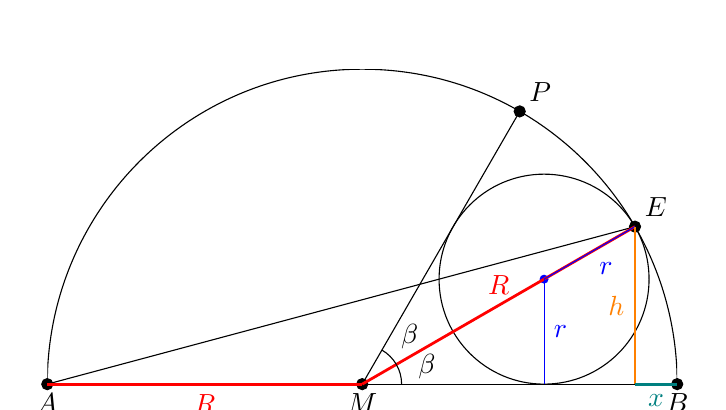
\begin{tikzpicture}[scale=4]
		% Koordinaten
		\coordinate (m) at (0,0);
		\coordinate (a) at (-1,0);
		\coordinate (b) at (1,0);
		\coordinate (p) at (0.5,0.866);
		\coordinate (e) at (0.866,0.5);
		\coordinate (kam) at (0.57732,0.33335);

		% Halbkreis
		\begin{scope}
			\clip (a) rectangle (1,1);
			\draw[black] (m) circle(1);
			\draw[black] (a) -- (b);
		\end{scope}

		% Kreis k_a
		\draw (kam) circle(0.33334);

		% Punkte
		\filldraw[black] (m) circle (0.5pt) node[anchor=north]{$M$};
		\filldraw[black] (a) circle (0.5pt) node[anchor=north]{$A$};
		\filldraw[black] (b) circle (0.5pt) node[anchor=north]{$B$};
		\filldraw[black] (p) circle (0.5pt) node[anchor=south west]{$P$};
		\filldraw[black] (e) circle (0.5pt) node[anchor=south west]{$E$};
		\filldraw[blue] (kam) circle (0.35pt);

		% Linien
		\draw[black] (a) -- (e);
		\draw[black] (m) -- (p);
		\draw[red, line width=1pt] (m) -- (e) node[midway,above]{$R$};
		\draw[red, line width=1pt] (a) -- (m) node[midway,below]{$R$};
		\draw[blue] (kam) -- (e) node[midway,below right]{$r$};
		\draw[blue] (kam) -- (0.57732,0) node[midway,right]{$r$};
		\draw[orange, line width=1pt] (e) -- (0.866,0) node[midway,left]{$h$};
		\draw[teal, line width=1pt] (b) -- (0.866,0) node[midway,below]{$x$};

		% Winkel
		\pic [draw,"$\beta$",angle eccentricity=1.7]{angle = b--m--e};
		\pic [draw,"$\beta$",angle eccentricity=1.7]{angle = e--m--p};
	\end{tikzpicture}
\end{center}

\begin{align*}
	m_{AE} &= \frac{\Delta y}{\Delta x} = \frac{h}{2R-x} \\
	\frac{h}{R} = \frac{r}{R-r} \leftrightarrow h &= \frac{Rr}{R-r} \tag{1} \\
	\Rightarrow m_{AE} &= \frac{Rr}{(2R-x)(R-r)}
\end{align*}

\begin{align*}
	\sin\beta &= \frac{\text{Gegenkathete}}{\text{Hypotenuse}} \tag{nötig?} \\
	&= \frac{r}{R-r} \\
	r &= R \sin\beta - r \sin\beta \\
	r + r \sin\beta &= R \sin\beta \\
	r(1+\sin\beta) &= R \sin\beta \\
	r &= \frac{R \sin\beta}{1 + \sin\beta} \tag{2}
\end{align*}

\begin{samepage}
	
	\begin{align*}
		\sin\beta &= \frac{\text{Gegenkathete}}{\text{Hypotenuse}} \\
		&= \frac{h}{R} \\
	\end{align*}
	mit $(1)$: \nopagebreak
	\begin{align*}
		\sin\beta &= \frac{Rr}{R(R-r)} \\
		&= \frac{r}{R-r} \\
		R-r &= \frac{r}{\sin\beta} \\
		R &= \frac{r}{\sin\beta}+r \\
	\end{align*}
	mit $(2)$: \nopagebreak
	\begin{align*}
		R &= \frac{R \sin\beta}{(1+ \sin\beta) \sin\beta} + \frac{R \sin\beta}{1 + \sin\beta} \\
		R &= 2 \frac{R \sin\beta}{1 + \sin\beta} \\
		R(1 + \sin\beta) &= 2 R \sin\beta \\
		R(1 + \sin\beta) - 2 R \sin\beta &= 0 \\
		R + R \sin\beta - 2 R \sin\beta &= 0 \\
		R &= R \sin\beta
	\end{align*}
\end{samepage}

\begin{center}
	\begin{tikzpicture}[scale=13]
		% Kreissektor mit 20°
		\draw[black] (m) -- (0:1) arc(0:20:1) -- cycle;

		% Punkte
		\coordinate (m) at (0,0);
		\coordinate (b) at (1,0);
		\coordinate (b2) at (0.93969,0.34202);
		\coordinate (p) at (0.98481,0.17365);
		\coordinate (p_) at (0.98481,0);
		\coordinate (kam) at (0.83896,0.14772);
		\coordinate (kam_side) at (0.98481,0.14772);

		\filldraw[black] (m) circle (0.25pt) node[anchor=east]{$M$};
		\filldraw[black] (p) circle (0.25pt) node[anchor=south west]{$P$};

		% Linien
		\draw[orange, line width=1pt] (p) -- (0.98481,0) node[midway,right]{$h$};
		\draw[red, line width=1pt] (m) -- (b2) node[midway,above left]{$R$};
		\draw[violet] (kam) -- (p) node[midway,above]{$r$};
		\draw[violet, line width=1pt] (kam) -- (0.83896,0) node[midway,left]{$r$};
		\draw[blue, line width=1pt] (m) -- (p_) node[midway,below]{$R_0$};
		\draw[teal, line width=1pt] (p_) -- (b) node[midway,below]{$x$};
		\draw[cyan, line width=1pt] (kam) -- (kam_side) node[midway,below]{$b$};
		\draw[black] (m) -- (p);

		% Kreis k_a
		\draw (kam) circle(0.14812);

		% Winkel
		\pic [draw,"$\beta$",angle eccentricity=2.6]{angle = b--m--b2};
		\pic [draw,"$\beta$",angle eccentricity=1.5]{angle = kam_side--kam--p};
	\end{tikzpicture}
\end{center}

\begin{align*}
	\textcolor{blue}{R_0} + \textcolor{teal}{x} &= \textcolor{red}{R} \\
	\frac{R_0}{h} &= \frac{R_0-b}{r} \\
	r R_0 &= h R_0 - hb \\
	r R_0 - h R_0 &= -hb \\
	R_0 (r-h) &= -hb \\
	R_0 &= \frac{-hb}{r-h}
\end{align*}

mit $ \cos\beta = \frac{b}{r} \Leftrightarrow b = r \cos\beta $ und $(1)$:

\begin{align*}
	R_0 &= \frac{\frac{-Rr}{R-r}*r \cos\beta}{r-\frac{Rr}{R-r}} \\
	&= \frac{\left(\frac{-Rr}{R-r}*r \cos\beta\right)}{\left(\frac{(R-r)r}{R-r}-\frac{Rr}{R-r}\right)} \\
	&= \frac{\left(\frac{-Rr}{R-r}*r \cos\beta\right)}{\left(\frac{Rr-r^2-Rr}{R-r}\right)} \\
	&= \frac{\left(\frac{-Rr^2 \cos\beta}{R-r}\right)}{\left(-\frac{r^2}{R-r}\right)} \\
	&= \frac{-Rr^2 \cos\beta * (R-r)}{-(R-r)r^2} \\
	&= R \cos\beta
\end{align*}

\begin{align*}
	R_0 + x &= R \\
	x &= R - R_0 \\
	&= R - R \cos\beta \tag{3}
\end{align*}

mit $(1)$ und $(3)$:

\begin{align*}
	m_{AE} &= \frac{h}{2R - x} \\
	&= \frac{\frac{Rr}{R-r}}{2R - (R-R \cos\beta)} \\
	&= \frac{\frac{Rr}{R-r}}{R+R \cos\beta} \\
	&= \frac{Rr}{(R-r)(R+R \cos\beta)} \\
	&= \frac{r}{(R-r)(1+\cos\beta)}
\end{align*}

mit $(2)$:

\begin{align*}
	m_{AE} &= \frac{\frac{R \sin\beta}{1+\sin\beta}}{(R-r)(1+\cos\beta)} \\
	&= \frac{R \sin\beta}{(R-r)(1+\cos\beta)(1+\sin\beta)} \\
	&= \frac{R \sin\beta}{(R-\frac{R \sin\beta}{1+\sin\beta})(1+\cos\beta)(1+\sin\beta)} \\
	&= \frac{R \sin\beta}{(\frac{R}{1+\sin\beta})(1+\cos\beta)(1+\sin\beta)} \\
	&= \frac{\sin\beta}{\frac{(1+\sin\beta)(1+\cos\beta)}{1+\sin\beta}} \\
	&= \frac{(\sin\beta)(1+\sin\beta)}{(1+\sin\beta)(1+\cos\beta)} \\
	&= \frac{\sin\beta}{1+\cos\beta}
\end{align*}

\pagebreak

\subsection[]{Herleitung von $m_{CD}$}
\fancyhead[L]{A3 --- $m_{CD}$}
Hierfür relevante Punkte und Strecken:

\begin{center}
	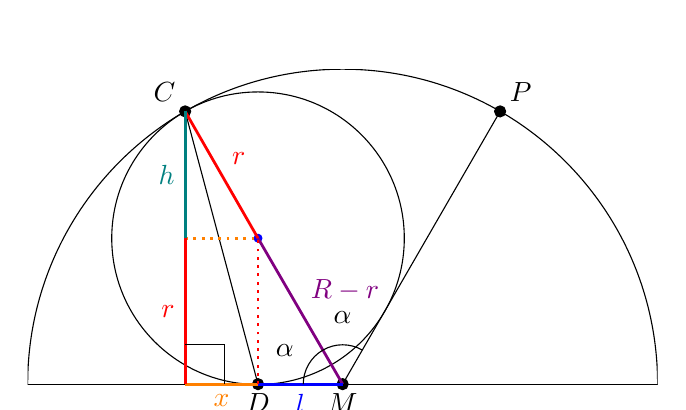
\begin{tikzpicture}[scale=4]
		% Koordinaten
		\coordinate (m) at (0,0);
		\coordinate (a) at (-1,0);
		\coordinate (b) at (1,0);
		\coordinate (p) at (0.5,0.866);
		\coordinate (c) at (-0.5,0.866);
		\coordinate (c_) at (-0.5,0);
		\coordinate (d) at (-0.26864,0);
		\coordinate (kbm) at (-0.26864,0.46335);
		\coordinate (kbm_side) at (-0.5,0.46335);

		% Kreis k_b
		\draw (kbm) circle(0.46441);

		% Halbkreis
		\begin{scope}
			\clip (a) rectangle (1,1);
			\draw[black] (m) circle(1);
			\draw[black] (a) -- (b);
		\end{scope}

		% Punkte
		\filldraw[black] (m) circle (0.5pt) node[anchor=north]{$M$};
		\filldraw[black] (d) circle (0.5pt) node[anchor=north]{$D$};
		\filldraw[black] (p) circle (0.5pt) node[anchor=south west]{$P$};
		\filldraw[black] (c) circle (0.5pt) node[anchor=south east]{$C$};
		\filldraw[blue] (kbm) circle (0.35pt);

		% Linien
		\draw[black] (m) -- (p);
		\draw[black] (c) -- (d);

		\draw[violet, line width=1pt] (m) -- (kbm) node[midway,above right]{$R-r$};
		\draw[red, line width=1pt] (kbm) -- (c) node[midway,above right]{$r$};
		\draw[blue, line width=1pt] (m) -- (d) node[midway,below]{$l$};
		\draw[orange, line width=1pt] (c_) -- (d) node[midway,below]{$x$};
		\draw[orange, dotted, line width=1pt] (kbm_side) -- (kbm) node[midway,below]{};
		\draw[red, line width=1pt] (c_) -- (kbm_side) node[midway,left]{$r$};
		\draw[red, dotted, line width=1pt] (d) -- (kbm) node[midway,left]{};
		\draw[teal, line width=1pt] (kbm_side) -- (c) node[midway, left]{$h$};

		% Winkel
		\pic [draw,"$\alpha$",angle eccentricity=1.7]{angle = p--m--c};
		\pic [draw,"$\alpha$",angle eccentricity=1.7]{angle = c--m--a};
		\pic [draw,angle eccentricity=1]{right angle = c--c_--m};
	\end{tikzpicture}
\end{center}

\begin{align*}
	m_{CD} &= \frac{\Delta y}{\Delta x} = \frac{h+r}{-x}
\end{align*}

\begin{align*}
	\textcolor{violet}{(R-r)}^2 &= \textcolor{red}{r}^2+\textcolor{blue}{l}^2 \\
	l &= \sqrt{(R-r)^2-r^2} \\
	&= \sqrt{R(R-2r)} \tag{1}
\end{align*}

\begin{align*}
	\sin\alpha &= \frac{ \textcolor{red}{r} }{ \textcolor{violet}{R-r} } \\
	r &= R\sin\alpha - r\sin\alpha \\
	r(1+\sin\alpha) &= R\sin\alpha \\
	r &= \frac{R\sin\alpha}{1+\sin\alpha} \tag{2}
\end{align*}

\begin{align*}
	\textcolor{teal}{h}^2 + \textcolor{orange}{x}^2 &= \textcolor{red}{r}^2 \\
	h &= \sqrt{r^2-x^2} \tag{3}
\end{align*}

\begin{align*}
	\frac{l}{r} &= \frac{l+x}{r+h} \\
	\text{mit (3):} \\
	\frac{l}{r} &= \frac{l+x}{r+\sqrt{r^2-x^2}} \\
	(r+\sqrt{r^2-x^2})l &= r(l+x) \\
	rl + l\sqrt{r^2-x^2} &= rl+rx \\
	l\sqrt{r^2-x^2} &= rx \\
	l^2(r^2-x^2) &= r^2 x^2 \\
	l^2 r^2 - l^2 x^2 &= r^2 x^2 \\
	r^2 x^2 + l^2 x^2 &= l^2 r^2 \\
	x^2 (r^2+l^2) &= l^2 r^2 \\
	x^2 &= \frac{l^2 r^2}{r^2 + l^2} \\
	x &= \frac{lr}{\sqrt{r^2+l^2}} \\
	&= \frac{lr}{R-r} \\
	\text{mit (1):} \\
	&= \frac{\sqrt{R(R-2r)}r}{R-r} \\
	\text{mit (2):} \\
	&= \frac{\sqrt{R(R-2\frac{R\sin\alpha}{1+\sin\alpha})}\frac{R\sin\alpha}{1+\sin\alpha}}{R-\frac{R\sin\alpha}{1+\sin\alpha}} \\
	&= \frac{\sqrt{R(R-2\frac{R\sin\alpha}{1+\sin\alpha})}\frac{R\sin\alpha}{1+\sin\alpha}}{\frac{R}{1+\sin\alpha}} \\
	&= \frac{R\sqrt{\frac{1-\sin\alpha}{1+\sin\alpha}}\frac{\sin\alpha}{1+\sin\alpha}}{\frac{1}{1+\sin\alpha}} \\
	x &= R\sin\alpha\sqrt{\frac{1-\sin\alpha}{1+\sin\alpha}} \tag{4}
\end{align*}

Weitergehend von $(3)$, mit $(2)$ und $(4)$:

\begin{align*}
	h &= \sqrt{r^2-x^2} \\
	&= \sqrt{\left(\frac{R\sin\alpha}{1+\sin\alpha}\right)^2 - \left(R\sin\alpha\sqrt{\frac{1-\sin\alpha}{1+\sin\alpha}}\right)^2} \\
	&= \sqrt{\frac{(R\sin\alpha)^2}{(1+\sin\alpha)^2} - \frac{(R\sin\alpha)^2(1-\sin\alpha)}{1+\sin\alpha}} \\
	&= \sqrt{\frac{(R\sin\alpha)^2}{(1+\sin\alpha)^2} - \frac{(R\sin\alpha)^2(1-\sin\alpha)(1+\sin\alpha)}{(1+\sin\alpha)^2}} \\
	&= \frac{\sqrt{(R\sin\alpha)^2(1-(1-\sin\alpha)(1+\sin\alpha))}}{1+\sin\alpha} \\
	&= R\sin\alpha \, \frac{\sqrt{1-(1-\sin\alpha)(1+\sin\alpha)}}{1+\sin\alpha} \\
	&= R\sin\alpha \, \frac{\sqrt{1-(1-\sin^2\alpha)}}{1+\sin\alpha} \\
	h &= R\sin\alpha \, \frac{\sin\alpha}{1+\sin\alpha} \tag{$3^\prime$}
\end{align*}

Mit $(2)$, $(3^\prime)$ und $(4)$:

\begin{align*}
	m_{CD} &= \frac{h+r}{-x} \\
	&= \frac{R\sin\alpha \frac{\sin\alpha}{1+\sin\alpha} + \frac{R\sin\alpha}{1+\sin\alpha}}{-R\sin\alpha\sqrt{\frac{1-\sin\alpha}{1+\sin\alpha}}} \\
	&= \frac{\frac{\sin\alpha+1}{1+\sin\alpha}}{-\sqrt{\frac{1-\sin\alpha}{1+\sin\alpha}}} \\
	&= -\sqrt{\frac{1+\sin\alpha}{1-\sin\alpha}} \\
	&= -\frac{\sqrt{1+\sin\alpha}}{\sqrt{1-\sin\alpha}} \\
	&= -\frac{\sqrt{1+\sin\alpha}\sqrt{1+\sin\alpha}}{\sqrt{1-\sin\alpha}\sqrt{1+\sin\alpha}} \\
	&= -\frac{1+\sin\alpha}{\sqrt{1 - \sin^2\alpha}} \\
	&= -\frac{\sin\alpha+1}{\sqrt{\cos^2\alpha}} \\
	&= -\frac{\sin\alpha+1}{\cos\alpha}
\end{align*}

\pagebreak
\fancyhead[L]{A3}
Für die Winkel $\alpha$ und $\beta$ gilt:

\begin{center}
	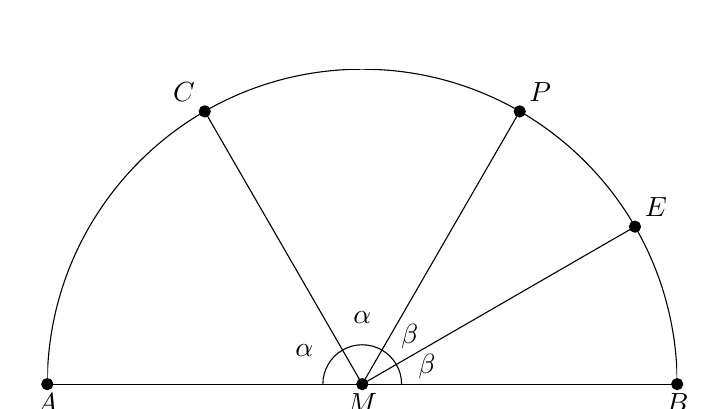
\begin{tikzpicture}[scale=4]
		% Punkte
		\coordinate (m) at (0,0);
		\coordinate (a) at (-1,0);
		\coordinate (b) at (1,0);
		\coordinate (p) at (0.5,0.866);
		\coordinate (c) at (-0.5,0.866);
		\coordinate (e) at (0.866,0.5);

		% Halbkreis
		\begin{scope}
			\clip (a) rectangle (1,1);
			\draw[black] (m) circle(1);
			\draw[black] (a) -- (b);
		\end{scope}

		% Punkte
		\filldraw[black] (m) circle (0.5pt) node[anchor=north]{$M$};
		\filldraw[black] (a) circle (0.5pt) node[anchor=north]{$A$};
		\filldraw[black] (b) circle (0.5pt) node[anchor=north]{$B$};
		\filldraw[black] (p) circle (0.5pt) node[anchor=south west]{$P$};
		\filldraw[black] (c) circle (0.5pt) node[anchor=south east]{$C$};
		\filldraw[black] (e) circle (0.5pt) node[anchor=south west]{$E$};

		% Linien
		\draw[black] (m) -- (p);
		\draw[black] (m) -- (c);
		\draw[black] (m) -- (e);

		% Winkel
		\pic [draw,"$\alpha$",angle eccentricity=1.7]{angle = p--m--c};
		\pic [draw,"$\alpha$",angle eccentricity=1.7]{angle = c--m--a};
		\pic [draw,"$\beta$",angle eccentricity=1.7]{angle = b--m--e};
		\pic [draw,"$\beta$",angle eccentricity=1.7]{angle = e--m--p};
	\end{tikzpicture}
\end{center}

\begin{align*}
	2\beta + 2\alpha &= \ang{180} \\
	\alpha &= \ang{90} - \beta \\
	\sin\alpha &= \sin(\ang{90} - \beta) = \cos\beta \\
	\cos\alpha &= \cos(\ang{90} - \beta) = \sin\beta \\
\end{align*}

So lässt sich $m_{CD}$ anders ausdrücken:

\begin{align*}
	m_{CD} &= -\frac{\sin\alpha+1}{\cos\alpha} \\
	&= -\frac{\cos\beta+1}{\sin\beta} \\
	m_{AE} &= \frac{\sin\beta}{\cos\beta+1}
\end{align*}

Somit gilt $ m_{CD} = -\frac{1}{m_{AE}} $, und damit auch: $CD \perp AE$.

\pagebreak
\section[]{Aufgabe 4}
\fancyhead[L]{A4}

\end{document}
